\documentclass{article} % For LaTeX2e
\usepackage{nips15submit_e,times}
\usepackage{hyperref}
\usepackage{cite}
\usepackage{url}
\usepackage[utf8]{inputenc}
\usepackage{amsmath}
\usepackage{amsfonts}
%\documentstyle[nips14submit_09,times,art10]{article} % For LaTeX 2.09
\usepackage{graphicx}
\usepackage{subfig}
\usepackage{graphicx}
\usepackage{epstopdf}
\epstopdfsetup{update}
\usepackage{float}

\title{SLT Project Report: Segmentation of neuron bundles from Diffusion MRI}


\author{
Antonio Orvieto \\
\texttt{orvietoa@student.ethz.ch} \\
\And
Sjoerd van Bekhoven \\
\texttt{vsjoerd@student.ethz.ch} \\
\And
Moisés Torres \\
\texttt{moisest@student.ethz.ch} \\
}

% The \author macro works with any number of authors. There are two commands
% used to separate the names and addresses of multiple authors: \And and \AND.
%
% Using \And between authors leaves it to \LaTeX{} to determine where to break
% the lines. Using \AND forces a linebreak at that point. So, if \LaTeX{}
% puts 3 of 4 authors names on the first line, and the last on the second
% line, try using \AND instead of \And before the third author name.

\newcommand{\fix}{\marginpar{FIX}}
\newcommand{\new}{\marginpar{NEW}}

\nipsfinalcopy % Uncomment for camera-ready version

\begin{document}


\maketitle

\begin{abstract}
As in any problem of this kind, the key to get good results is to understand how the data is generated and how specific biological properties are translated into the numbers we see in our files. In this report we are going to explore a particular similarity measure to solve the bundle segmentation problem with superparamagnetic clustering. This only has to be considered as a starting point for some possible further work on the subject, and not as a solution of the problem. Details about our doubts and difficulties will be covered in the report.
\end{abstract}

\section{The Diffusion Tensor}
Let us start from the beginning: for  every point $(x,y,z)$ in the brain, we are given measurements about the water diffusion at that point. The \texttt{nii} file combined with the \texttt{bvecs} gives us the diffusion
\footnote{Actually we are given a signal which is inverse proportional to the diffusion. Hence the maximum diffusion direction is the minimum signal direction.} 
strength at that point (voxel), sampled at $164$ directions (however 20 of them are not valid). Our task is to segment neuron bundles using this diffusion information.
As it is very well described in \cite{Mukherjee01042008}, white matter tracts in the brain are characterized\footnote{This is not actually true at fiber crossings} by a strongly anisotropic diffusion in the direction of the fiber, whereas grey matter, CSF spaces and basically any other part of the brain has isotropic diffusion. 

In Figure 1 one can see how different the diffusion is when the signal comes from a white matter voxel (b) or not (a).

\begin{figure}[H]
  \centering
  \subfloat[Isotropic case: p=(63,46,1) ]{\includegraphics[width=0.4\textwidth]{img/FA005.png}\label{fig:f1}}
  \hfill
  \subfloat[Anisotropic case: p=(63,46,26).]{\includegraphics[width=0.4\textwidth]{img/FA076.png}\label{fig:f2}}
  \caption{Different modes of diffusion.}
\end{figure}


Moreover, diffusion is a random transport phenomenon, furthermore the diffusion signals can be elegantly modeled by a Multivariate Normal Distribution in $\mathbb{R}^3$  \cite{Alexander2007,basser:1994:eesd}: the maximum diffusion direction corresponds to the eigenvector associated with the largest eigenvalue (all of them are positive) of the covariance matrix of this distribution. This model is reasonable because:
\begin{enumerate}
\item Water diffusion is related to Brownian Motion and therefore to the normal distribution.
\item The shape of our samples from this distribution (i.e. our data for every voxel) is very similar to an ellipsoid.
\end{enumerate}
In order to get some intuition about the latter (hence to get the plots in Figure 1), we loaded the whole \texttt{nii} file on MATLAB and we used the \texttt{Ellipsoid fit} library \footnote{\url{http://ch.mathworks.com/matlabcentral/fileexchange/24693-ellipsoid-fit}}  
to get an estimate of the eigenvectors and eigenvalues of the covariance matrix at each voxel. After that (the procedure only takes a couple of hours in a regular laptop for the whole dataset) we computed for every voxel a quantity called Fractional Anisotropy\cite{Peeters2009,Mukherjee01042008}: let $\lambda_1, \lambda_2, \lambda_3$ be the eigenvalues of an ellipsoid:
\begin{equation}
FA = \frac{\sqrt{(\lambda_1-\lambda_2)^2+(\lambda_3-\lambda_2)^2+(\lambda_1-\lambda_3)^2}}{\sqrt{2(\lambda_1^2+\lambda_2^2+\lambda_3^2)}}.
\end{equation}
The Fractional Anisotropy is 0 if the ellipsoid is actually a sphere (completely isotropic) and is 1 in the extreme anisotropic case: this quantity is very convenient to identify the strong diffusion areas of the brain. In Figure 2 you can see a slice of the brain at $x=60$, where the red pixels have a fractional anisotropy greater than $0.34$ (this is a bit high and some white matter is of course not plotted).   

\begin{figure}[H]
  \centering
{\includegraphics[width=0.4\textwidth]{img/k0_34.PNG}\label{F}}
\caption{White matter at the section x=60, $FA > 0.34$}
\end{figure}

Now we should ask ourselves a crucial question: how do I identify a fiber? There are several methods to do that, most of them are described in \cite{Mukherjee01042008}.
However we are going to use pairwise clustering, in particular Blatt's super-paramagnetic clustering technique\cite{Blatt1997}. The only parameter we can choose in the algorithm is the $J_{ij}$, which is the cost of \underline{not} assigning the voxel $i$ and the voxel $j$ to the same fiber (cluster): $J_{ij}$ should be high when $i$ and $j$ are similar (so we want to keep them in the same cluster) and should be small when $i$ and $j$ are not similar. But how do we measure similarity between ellipsoids? \\
Many approaches exist right now to do this, and most of them depend on the application: a good list of such similarity measures can be found in \cite{Peeters2009}. However, we are going to use the simplest of them: for every voxel we only keep the maximum diffusion (minimum signal) direction, and then we compute $J_{ij}$ as a simple function of the angle between the vectors: let $v_i$ and $v_j$ be the maximum diffusion directions of the voxels $i$ and $j$ respectively, we define:
\begin{equation}
J_{ij}= \exp\left[-k \left(\frac{\langle vi, vj \rangle}{||v_i|| \ ||v_j||}\right)^2\right].
\end{equation}
Where we set $k=6$ (it appears to work, but maybe it needs to be tuned in properly, maybe with some local considerations like the parameter $a$ in \cite{Blatt1997}). $J_{ij}$ is (almost) 0 for orthogonal diffusion directions, and it is 1 for parallel diffusion directions. Moreover we will only consider in our clustering points with relatively high fractional anisotropy (not too high, as we would loose the fiber structure). This has of course both drawbacks and advantages. We start enumerating the advantages:

\begin{enumerate}
\item Data compression (i.e. get minimum signal direction) can be done in MATLAB\footnote{We do this fitting the ellipsoid with the previous library. Unfortunately such a library does not exist for Python and it is really difficult to program: the ellipsoid fitting problem for dimension 3 or more is a well known challenging problem, further reference can be found in \cite{Ellips}} before the clustering procedure.
\item The computation of the $J_{ij}$ is trivial at each step.  Moreover the Fractional Anisotropy threshold eliminates a lot of points, making the computation faster.
\item Considering just the diffusion directions (and not lengths for example) is convenient as the diffusivity in the brain is not constant and depends on the individual \cite{Alex}.
\item The method can be easily validated, as can be seen in the last section.
\end{enumerate}

However the method does have some serious drawbacks:

\begin{enumerate}
\item It is not clear whether our compression results in less robustness: in our opinion this is not really a big problem, as not completely anisotropicity is not due to the noise, but rather to the MRI technology.
\item This method fails when dealing with crossing fibers. Further information can be found in \cite{Gee2006}
\item Other similarity measures could perform way better than this. In the future we would definitely love to experiment with the Pollari distance measure \cite{4193399}
\end{enumerate}

\section{Super-paramagnetic Clustering}

For our clustering algorithm, we have implemented the (nonparametric) procedure described in Blatt's 1997 paper \cite{Blatt1997}.  Algorithms such as histogram clustering (which is parametric) will fail, if not modified correctly, to capture the connectedness property required for the fibers as it only considers the statistics of each point in isolation.

The main idea for the selected approach is to model our data by using a Potts model. Each data point is assigned a Potts spin and then an interaction between neighboring points is introduced. This magnetic system will exhibit three different phases: ferromagnetic, super-paramagnetic and paramagnetic. In the intermediate regime (super-paramagnetic) clusters of relatively strongly coupled spins become ordered, whereas different clusters remain uncorrelated. We will take advantage of this property to perform the clustering of the data.

\subsection{Potts model simulation: Swendsen-Wang algorithm}

In order to identify the range of temperatures corresponding to the super-paramagnetic regime, we make use of the fact that when at this phase, the magnetic system will experiment a jump in the order parameters. Specifically, a sharp transition between the ferromagnetic and the super-paramagnetic regimes is observed in the susceptibility $\chi$:

\begin{equation}
\chi=\frac{N}{T}(\langle m^2 \rangle - \langle m \rangle^2)
\end{equation}

In the above formula can be seen that the susceptibility is related to the variance of another thermal quantity, the magnetization $\langle m \rangle$:

\begin{equation} \label{eq:boltz}
\langle m \rangle = \sum_{\mathcal{S}}m(\mathcal{S})P(\mathcal{S})\quad \text{with}\quad P(\mathcal{S})=\frac{1}{Z}\ exp(-\frac{\mathcal{H}(\mathcal{S})}{T}),\ m(\mathcal{S})=\frac{qN_{max}(\mathcal{S})-N}{(q-1)N}
\end{equation}

To obtain the magnetization, the thermal average of the magnetization over all possible spin configurations $\mathcal{S}$ has to be calculated. Direct evaluation of this sum is intractable, since the number of configurations increases exponentially with the size of the data ($q^N$).

To overcome this problem, we will use the Swendsen-Wang (SW) Monte Carlo simulation method (details on how to use our code are described in the \texttt{README.md} file). Basically we will sample possible configurations out of the set $\mathcal{S}$ according to the Boltzmann probability distribution from \eqref{eq:boltz}. Then the magnetization calculation turns out to be simply the average over the sampled configurations:

\begin{equation}
\langle m \rangle \approx \frac{1}{M} \sum_{i=1}^{M} m(\mathcal{S}_{i}) \quad \text{with} \quad \mathcal{S}_i \in \{\mathcal{S}_1, \mathcal{S}_2, ...,\mathcal{S}_M \}
\end{equation}

In order to construct such configurations, the SW algorithm proposes the following steps for each one of the temperatures:
\begin{enumerate}
\item Initialize the value of the Potts spins at random.
\item For all neighbouring points\footnote{Instead of letting all pairs interact, K-nearest neighbors are used due to computational reasons.}, establish a bond with probability:
\begin{equation}
p_{i,j}^{f}=1 - exp(-\frac{J_{i,j}}{T}\ \delta_{i,j})
\end{equation}
\item Find the connected subgraphs, the SW-clusters.
\item Generate a new Monte Carlo step by assigning a random spin value to all the nodes in the same cluster.
\item Calculate the magnetization of the new configuration.
\item Go to step 2 until the number of iterations is reached.
\item Average the magnetization obtained for each configuration.
\end{enumerate}

To improve the efficiency of the algorithm, it is straightforward to perform the simulation of each temperature in parallel as they are completely independent of each other. In our implementation, we used the Python package \texttt{joblib} to achieve this. With this improvement our code was able to take advantage of the large number of cores available at the Euler cluster (which we used to run the Monte Carlo simulations), speeding up the runtime notably.

We can see that through our simulation procedure we have been able to obtain an estimate of the susceptibility $\chi$ as a function of the temperature $T$, which reflects the thermodynamic phases of the system. Hence, we can identify the range of temperatures in which our system is in the super-paramagnetic regime and use this information to perform the clustering of our data.

\subsection{Clustering the data}
As we mentioned in the beginning, in the super-paramagnetic regime clusters of relatively strongly coupled spins become ordered. Thus, for our final step we will perform another Monte Carlo simulation to estimate the behaviour of our system in this phase. We will select an adequate temperature based on the previously obtained plot of the susceptibility, and for this temperature, we will use the SW algorithm described earlier. In this case, for each Monte Carlo step we will measure the two-point connectedness $C_{ij}$, which is the probability that two nodes belong to the same cluster. To calculate it we just keep track of the number of times that two nodes were in the same cluster in the different Monte Carlo steps and take the average at the end. Once we have this, we perform the clustering in the following way:
\begin{enumerate}
\item First, we build the "core" of the clusters by bonding the nodes with $C_{ij}>0.5$\footnote{Although in the Blatt paper \cite{Blatt1997} the spin-to-spin correlation $G_{ij}$ is used instead of $C_{ij}$, the authors also mention that is completely equivalent and that they only do it for didactic purposes.}. As mentioned in the Blatt paper \cite{Blatt1997}, the result depends weakly on this threshold.
\item Capture nodes lying on the periphery of the clusters, by linking them to the neighbour with highest $C_{ij}$.
\item The resulting subgraphs conform the clustering of the given data.
\end{enumerate}

\section{Results} 
For the results of the simulation in this section, we use a subset of $26 \times 26 \times 26 = 17576$ voxels with $x \in [50,75]$, $y \in [80,105]$ and $z \in [55,80]$. The number of iterations in the SW Monte Carlo model is 400 per temperature with 50 burn-in samples, ranging over 100 temperatures from $T = 0$ to $T = 1$. As mentioned before, we set a threshold on the fractional anisotropy (FA), in this case $\text{FA} > 0.25$. This leaves us a with a total of $N = 8942$ voxels. Each voxel interacts with its 10-neighborhood, which results in $\sim 60.000$ ($i,j$) interactions in total. The results of the Monte Carlo simulation of Potts models with the Swendsen-Wang method with the above settings can be found in Figure~\ref{fig:phase}.

When looking at the plot of the susceptibility density $\chi^T/N$, we find a strong peak at $T = 0.41$ which indicates a ferromagnetic to super-paramagnetic transition, or more informally the moment that a large cluster breaks into several still rather large clusters. This transition can also be spotted in the magnetization plot, which suddenly diminishes at $T = 0.41$.

For the transition from super-paramagnetic to paramagnetic, we look for a sudden decrease, which we find at about $T = 0.54$. From the susceptibility density plot, we therefore identify the the super-paramagnetic phase to be from $T = 0.41$ to $T = 0.54$. Note that between $T = 0.46$ and $T = 0.54$ a plateau can be spotted, which indicates large, stable clusters. Therefore, we pick a temperature in the plateau (which is in the super-paramagnetic phase) to create a clustering, in this case $T = 0.49$.

The results of the clustering at $T = 0.49$ can be found in Figure~\ref{fig:clusteringdist} and Figure~\ref{fig:clustering}. Figure~\ref{fig:clusteringdist} shows the distribution of the voxels over the clusters. In total, we found 1044 clusters of which 6 have a size larger than 200. These are plotted in Figure~\ref{fig:clustering}. We can clearly see some ``stripes'' that could very well denote fibers, such as for example the yellow and red cluster. To verify whether this indeed is the case, we validate our model in the next section.

\begin{figure}[H]
  \begin{center}
    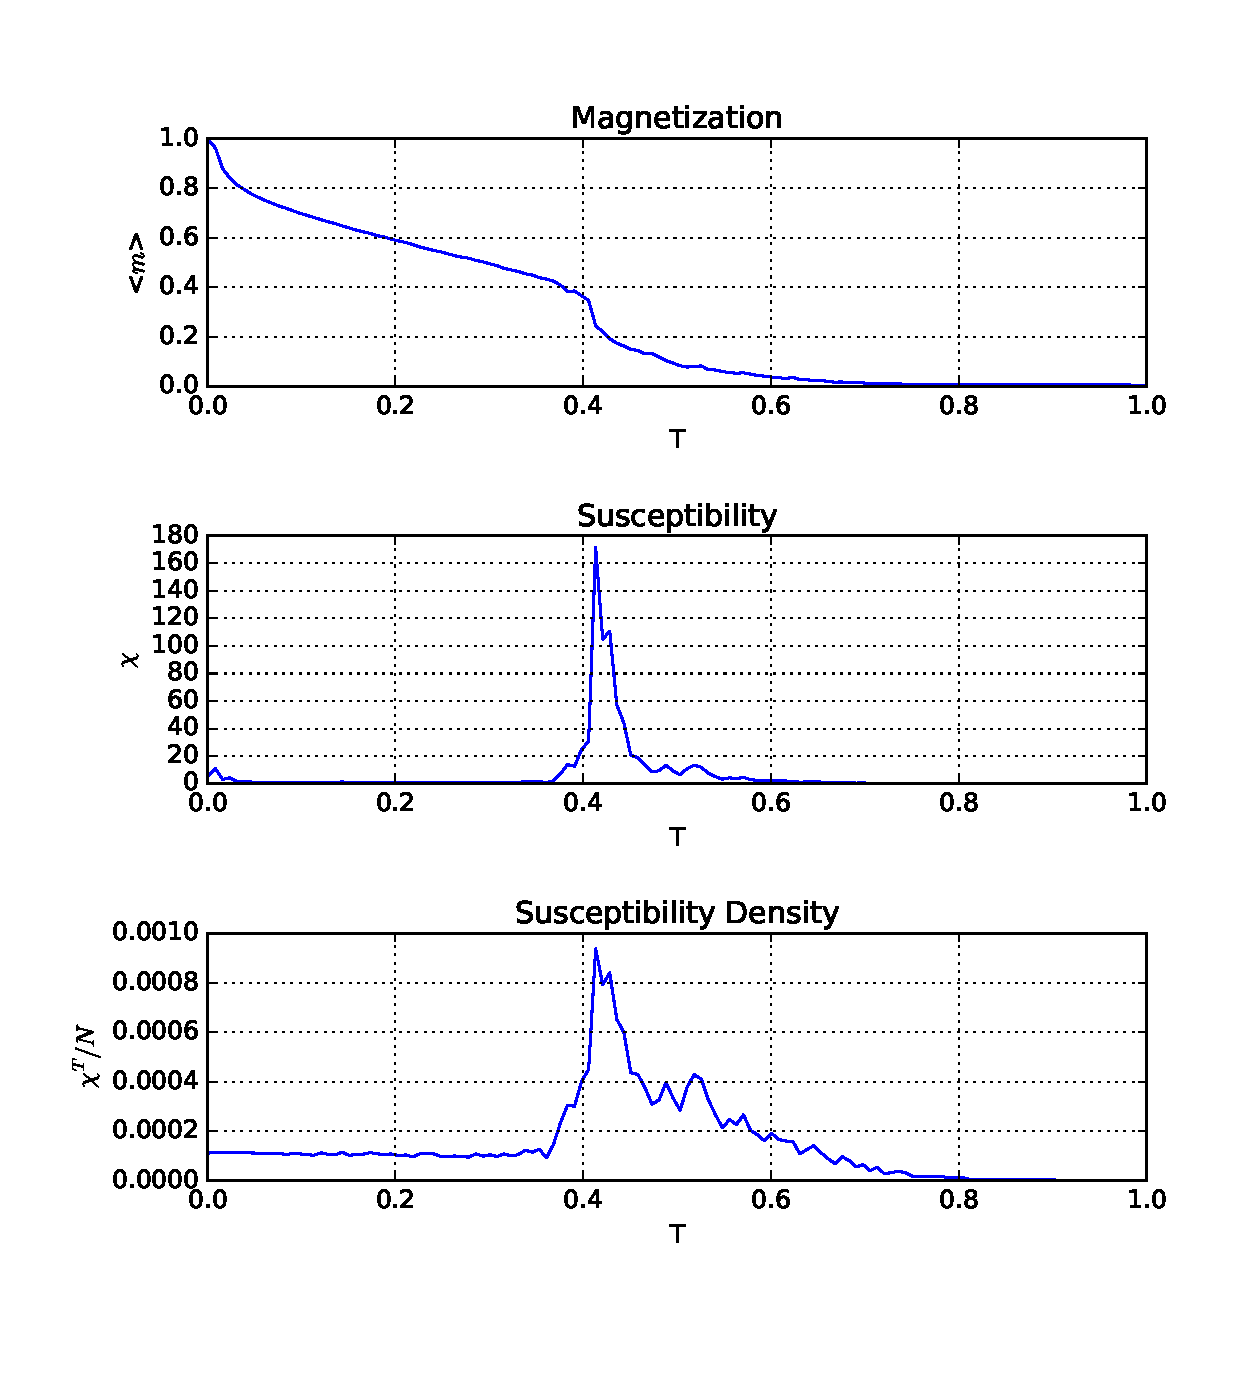
\includegraphics[width=\textwidth]{img/phase_analysis_subset_2_v2.eps}
  \end{center}
  \caption{Results of the Monte Carlo simulation of Potts models with the Swendsen-Wang method}
	\label{fig:phase}
\end{figure}

\begin{figure}[H]
  \begin{center}
    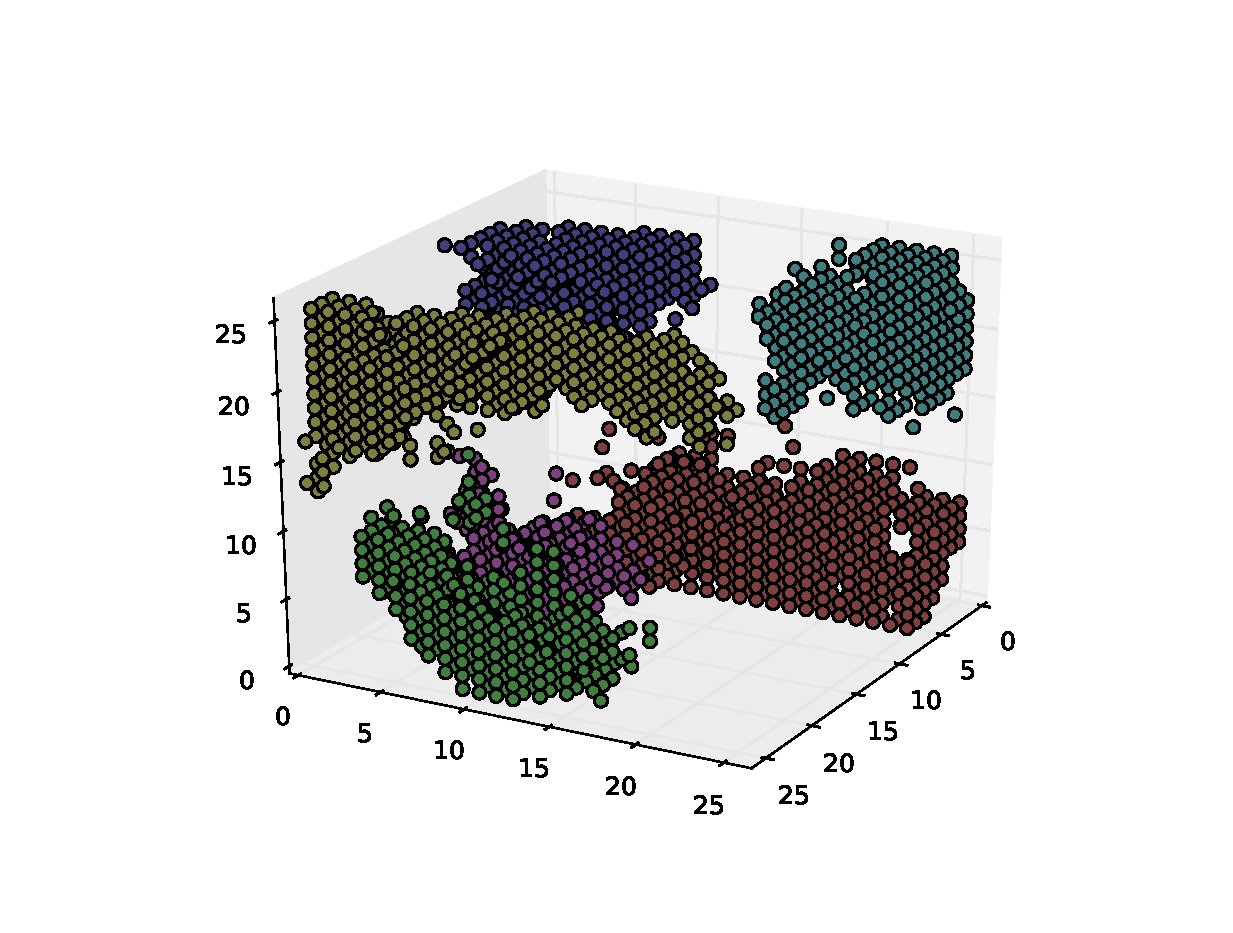
\includegraphics[width=\textwidth]{img/clustering.eps}
  \end{center}
  \caption{Clustering}
  \label{fig:clustering}
\end{figure}

\begin{figure}[H]
  \begin{center}
    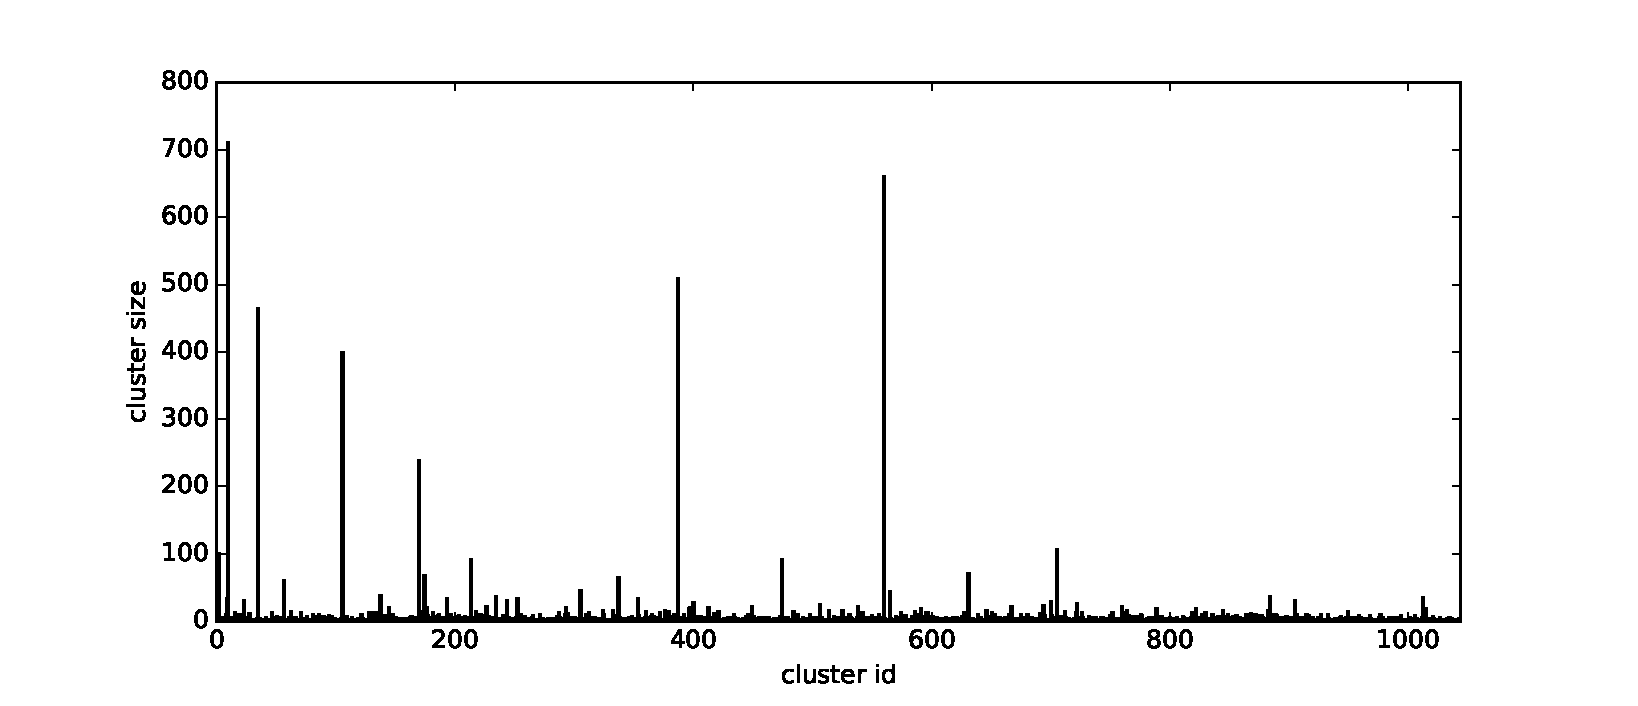
\includegraphics[width=\textwidth]{img/cluster_size.eps}
  \end{center}
  \caption{Cluster Distribution}
  \label{fig:clusteringdist}
\end{figure}

\section{Validation}
Now that we have established a clustering, we ask our selves: do the clusters actually denote fibers? Since the answer to this is generally unknown for this dataset, we at least verify our methodology. In this final section we attempt to do so by validating the results of a clustering with respect to the cost function we have constructed.

The cost function $J_{ij}$ used in the clustering algorithm is constructed in such a way that it prefers parallel maximum diffusion direction and is thus averse of clustering datapoints with orthogonal maximum diffusion direction. To verify that the clustering is in correspondence with this behavior, we look at a 2D slice of the dataset ($x=67$, $y \in [20,79]$ and $z \in [50,90]$), so that we can easily visualize the maximum diffusion direction by means of an arrow. An example of such a visualization can be found in Figure~\ref{fig:arrows}, only showing the datapoints with a fractional anisotropy of $\text{FA} > 0.25$, just as in our original results. In this figure, one can somewhat manually classify the fibers by following the arrows.

Now, let us look at the result of our clustering algorithm on the same slice of data, which can be found in Figure~\ref{fig:arrows_clustered}. In the clustering, a very large part of the datapoints is clustered together, but there are several, significantly smaller clusters. If we focus on the yellow cluster at the bottom right, we can clearly see that the datapoints that are separated from the big red cluster are denoted by vectors that are orthogonal to the vectors denoting the datapoints in the big red cluster close to them. If we look at other small clusters, we see similar behaviour. On the other hand, one can also pinpoint sections in the red cluster that contain datapoints that are denoted by orthogonal vectors, which ideally should not happen.

\begin{figure}[H]
  \begin{center}
    \includegraphics[width=0.7\textwidth]{img/2.png}
  \end{center}
  \caption{Maximum diffusion directions for 2D slice of the brain}
  \label{fig:arrows}
\end{figure}

\begin{figure}[H]
  \begin{center}
    \includegraphics[width=0.75\textwidth,height=0.25\textheight]{img/1.png}
  \end{center}
  \caption{Clustering for the previous slice}
  \label{fig:arrows_clustered}
\end{figure}

Another, more general way of validating our results, could be verifying whether the largest clusters in our clustering contain the majority of what we consider white matter for higher thresholds of the fractional anisotropy. For example, we have used only datapoints with $\text{FA} > 0.25$ for the subset in our experiments. By increasing this threshold, we will capture datapoints of which we are, by our previous assumptions, more and more sure that they are white matter. By comparing these datapoints with the datapoints in our clusters created for threshold $\text{FA} > 0.25$, our clustering can be considered ``good'' if it keeps a somewhat steady ratio of captured datapoints. Such a plot can be found in Figure~\ref{fig:validation} in which we can see that the number of datapoints captured by our 6 biggest clusters decreases way less steep than the total number of datapoints that we, by our assumptions, consider white matter.

\begin{figure}[H]
  \begin{center}
\includegraphics[width=0.75\textwidth,height=0.25\textheight]{img/validation.eps}
  \end{center}
  \caption{Validation with total number of white matter vs. the white matter covered by the 6 biggest clusters}
  \label{fig:validation}
\end{figure}

To sum up, with these examples we just try to get some insight of whether or not the designed cost function $J_{ij}$ succeeds in modeling both the connectedness and diffusion direction properties that characterize white matter tracts. However this only gives us an intuition of the correctness of our algorithm. More rigorous ways of validating tractography results are still a matter of research.




\small{

\bibliography{references} 
\bibliographystyle{ieeetr}

}



\end{document}
